\documentclass[a4paper]{artikel1}
\usepackage{lmodern}
\usepackage{amssymb,amsmath}
\usepackage{ifxetex,ifluatex}
\usepackage{fixltx2e} % provides \textsubscript
\ifnum 0\ifxetex 1\fi\ifluatex 1\fi=0 % if pdftex
  \usepackage[T1]{fontenc}
  \usepackage[utf8]{inputenc}
\else % if luatex or xelatex
  \ifxetex
    \usepackage{mathspec}
  \else
    \usepackage{fontspec}
  \fi
  \defaultfontfeatures{Ligatures=TeX,Scale=MatchLowercase}
  \newcommand{\euro}{€}
\fi
% use upquote if available, for straight quotes in verbatim environments
\IfFileExists{upquote.sty}{\usepackage{upquote}}{}
% use microtype if available
\IfFileExists{microtype.sty}{%
\usepackage{microtype}
\UseMicrotypeSet[protrusion]{basicmath} % disable protrusion for tt fonts
}{}
\usepackage[margin=1in]{geometry}
\usepackage{hyperref}
\PassOptionsToPackage{usenames,dvipsnames}{color} % color is loaded by hyperref
\hypersetup{unicode=true,
            pdftitle={Biotic invasions fuck with the manageability of pollination networks},
            pdfsubject={Supporting Information},
            pdfborder={0 0 0},
            breaklinks=true}
\urlstyle{same}  % don't use monospace font for urls
\usepackage{graphicx,grffile}
\makeatletter
\def\maxwidth{\ifdim\Gin@nat@width>\linewidth\linewidth\else\Gin@nat@width\fi}
\def\maxheight{\ifdim\Gin@nat@height>\textheight\textheight\else\Gin@nat@height\fi}
\makeatother
% Scale images if necessary, so that they will not overflow the page
% margins by default, and it is still possible to overwrite the defaults
% using explicit options in \includegraphics[width, height, ...]{}
\setkeys{Gin}{width=\maxwidth,height=\maxheight,keepaspectratio}
\setlength{\parindent}{0pt}
\setlength{\parskip}{6pt plus 2pt minus 1pt}
\setlength{\emergencystretch}{3em}  % prevent overfull lines
\providecommand{\tightlist}{%
  \setlength{\itemsep}{0pt}\setlength{\parskip}{0pt}}
\setcounter{secnumdepth}{0}

%%% Use protect on footnotes to avoid problems with footnotes in titles
\let\rmarkdownfootnote\footnote%
\def\footnote{\protect\rmarkdownfootnote}

%%% Change title format to be more compact
\usepackage{titling}

% Create subtitle command for use in maketitle
\newcommand{\subtitle}[1]{
  \posttitle{
    \begin{center}\large#1\end{center}
    }
}

\setlength{\droptitle}{-2em}
  \title{Biotic invasions fuck with the manageability of pollination networks}
  \pretitle{\vspace{\droptitle}\centering\huge}
  \posttitle{\par}
\subtitle{Supporting Information}
  \author{}
  \preauthor{}\postauthor{}
  \date{}
  \predate{}\postdate{}


\usepackage{setspace}
\usepackage{float}
\usepackage{rotating}
\renewcommand{\figurename}{Supporting Figure}
\renewcommand{\tablename}{Supporting Table}

% Redefines (sub)paragraphs to behave more like sections
\ifx\paragraph\undefined\else
\let\oldparagraph\paragraph
\renewcommand{\paragraph}[1]{\oldparagraph{#1}\mbox{}}
\fi
\ifx\subparagraph\undefined\else
\let\oldsubparagraph\subparagraph
\renewcommand{\subparagraph}[1]{\oldsubparagraph{#1}\mbox{}}
\fi

\begin{document}
\maketitle

\doublespacing

\section{S1: Finding a complex network's
matchings}\label{s1-finding-a-complex-networks-matchings}

Our approach to find the minumum number of driver nodes relies on
finding maximum matchings and maximum cardinality matchings. Most
existing algorithms are designed to work with undirected bipartie
networks, where finding the maximum matching is equivalent to finding
the maximum flow between the two levels.

We start with a directed network in which the direction of the link
represents the direction of control (Supporting figure 1a). We then
construct an alternative representation of the directed network in which
each node of the directed network is represented by two nodes that
indicate their outgoing and incoming links (Supporting figure 1b).
Finding a maximum matching in this alternative representation is
equivalent to finding the largest possible set of edges in which one
node in the left hand side is connected to at most one node in the right
hand side. To find the maximum matching we use the push-relabel
algorithm implemented in \texttt{max\_bipartite\_matching} in the R
package igraph 1.0.1 (Csardi \& Nepusz 2006). Once we have the matching
shown in the Supporting Figure 1b, it is then easy to identify the roles
of each node in this representation: nodes on the right hand side that
are connected to a matched link (purple) are matched, while those
connected to a matched link on the left hand side are superior. This
information can then be mapped back to the original representation to
identify the control paths and the driver nodes in the network
(Supporting Figure 1c). Supporting Figure 1d, e, and f ilustrate this
approach for a network with bidirectional links.

\begin{figure}[htbp]
\centering
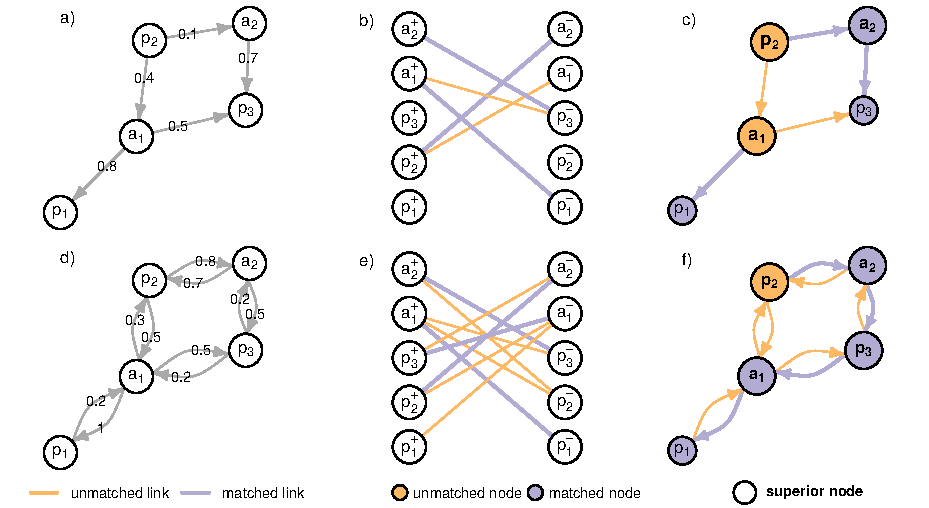
\includegraphics{supp_info_2_files/figure-latex/fig-direction-of-control-1.pdf}
\caption{\textbf{Finding a maximum matching in a complex network}. (a \&
d) Directed networks that indicate the direction of control between
species. (b \& e) Alternative bipartite representations of the directed
networks. (c \& f) The matchings in the bipartite representation mapped
back to the original network.}
\end{figure}

The algorithm implemented in \texttt{max\_bipartite\_matching}, however,
is only able to find \textbf{one} of the, possibly many, maximum
matchings in a network. One maximum matching is sufficient to calculate
\emph{n\textsubscript{D}} and hence to provide indication of a
communitie's manageability, however it is not possible to estimate the
role of individual species. To do that we need to calculate all possible
maximum matchings (or all maximal cardinality matchings in weighted
networks like ours). We start from the alternative bipartite
representation in Supporting Figure 1b and assign an identity to each of
the links in the network (shown as numbers in Supporting Figure 2a). We
will call this bipartite representation \emph{B}. We then construct the
line graph of the alternative bipartite representation \emph{L(B)}
(Supporting Figure 2b). Each node in \emph{L(B)} represents a link in
\emph{B} and are connected to each other only if they share a common
node in \emph{B}. We calculate the complement graph of \emph{L(B)} and
idetify all the maximum cliques (Supporting Figure 2c). Here some extra
definitions are neccessary. First, the complement of \emph{L(B)},
\emph{H}, is a graph with the same nodes as \emph{L(B)} but that has a
link between two given nodes if and only if there is not a link in
\emph{L(B)}. Second, a clique is a subset of nodes such that any two of
them are linked. Lastly, a maximum clique is a clique such that there
are no cliques with more nodes. In this example there are two maximum
cliques: that one formed by 1, 3 and 5, and by 2, 3 and 5. The final
step is then to map these cliques into the original network to obtain
all possible maximum cardinality matchings as shown in Figure 1 in the
main text.

\begin{figure}[htbp]
\centering
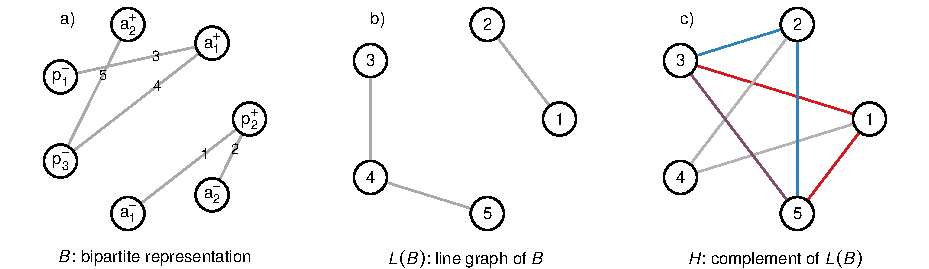
\includegraphics{supp_info_2_files/figure-latex/fig-finding-all-matchings-1.pdf}
\caption{\textbf{Finding all possible maximum cardinality matchings}.
(a) Alternative bipartite representation of a directed network. (b) Line
graph of the network in a. (c) Complement of the network in b. The two
maximum cliques are shown in red and blue.}
\end{figure}

In the main text we show all maximum cardinality matchings for a simple
example network. To further ilustrate our methodology, here we also show
the approach for the smallest of our empirical networks, the uninvaded
network at site 10 (Supporting Table 1; Supporting Figure 3). The
largest component of this network is composed by 16 species of which 2
are non-invasive plants and the rest are pollinators. The one-to-one
relationship between matched and superior nodes implies that in order to
achieve full network controllability, most pollinators would be
unmatched, and hence driver species that require external intervention.
At the same time, both plants in the community, \emph{Heracleum
sphpndylum} and \emph{Rubus fructicosus} and one of the pollinators
\emph{Orthotylus/Lygocorus} tend to be classified as superior nodes.

\begin{figure}[htbp]
\centering
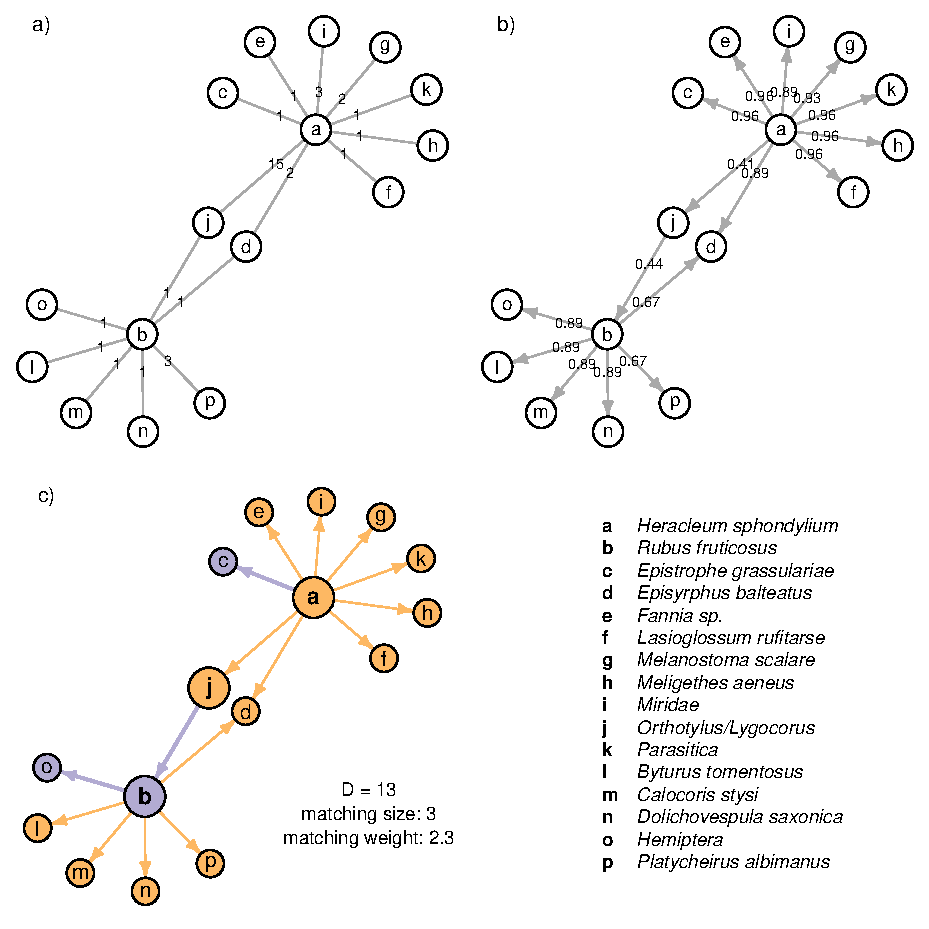
\includegraphics{supp_info_2_files/figure-latex/fig-SA_exp-1.pdf}
\caption{\textbf{Illustration of the procedure with one empirical
network}. (a) The initial visitation network. (b) The directed network
in which the direction of control and the magnitude of the asymmetry are
determined based on the mutual dependences. (c) One of the possible
maximum matchings calculated using the procedures illustrated in the
Supporting Figure 1 and 2.}
\end{figure}

In addition, here we also show all the maximum cardinality matchings for
an example network in which the links are bidirectional (Supporting
Figure 4). It is important to note that using bidirectional is
problematic for a couple

It is important to note that our approach to find all the maximum
matchings, which is based on the alternative bipartite representation of
the directed network and a series of network transofrmations, has an
important disadvantage. Namely, that it is possible tha cycles in
network figure 4

\begin{figure}[htbp]
\centering
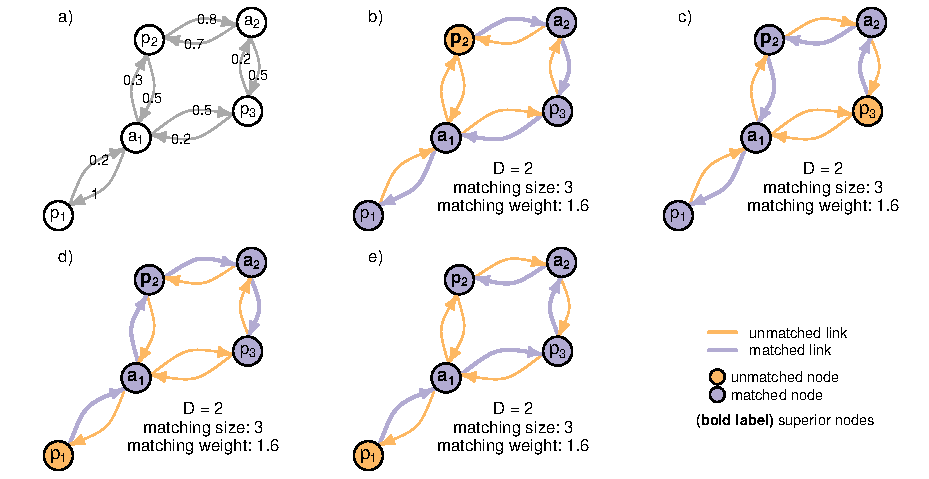
\includegraphics{supp_info_2_files/figure-latex/fig-matchings-bidirectional-1.pdf}
\caption{SAD}
\end{figure}

\begin{figure}[htbp]
\centering
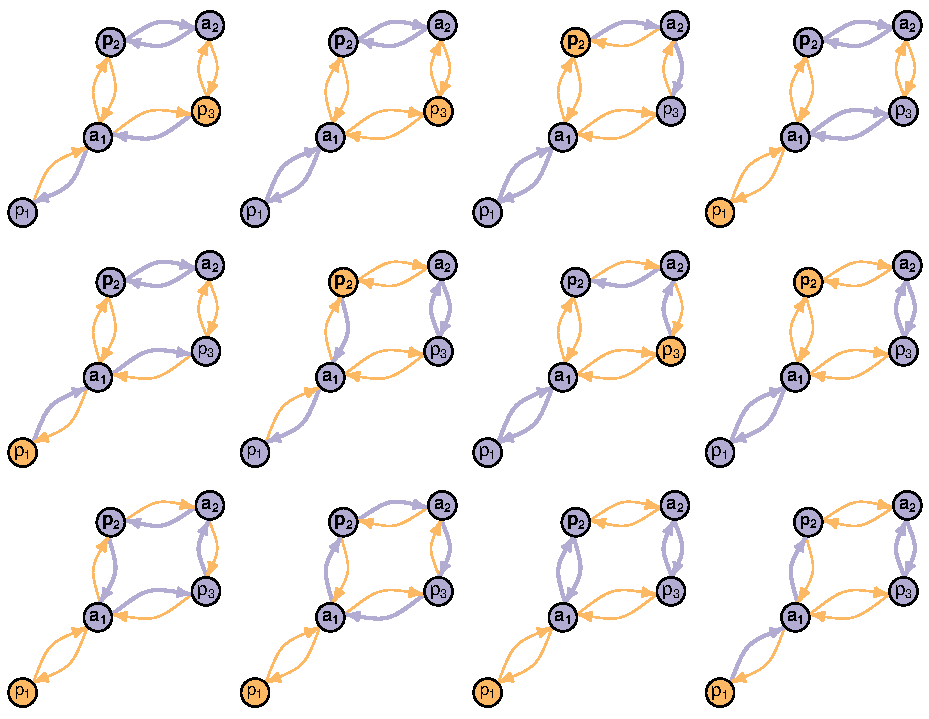
\includegraphics{supp_info_2_files/figure-latex/fig-matchings-bidirectional-no-1.pdf}
\caption{asd asd}
\end{figure}

\section{S2: Properties of empirical
networks}\label{s2-properties-of-empirical-networks}

The studied networks had species richess ranging between 19 and 87
(16-86 when considering only the largest component in each network). As
evidenced by the overall network asymmetry \emph{AS} (Blüthgen \emph{et
al.} 2007) networks had a low ratio of plants to pollinators.
Furthermore, networks had relatively low levels of nestedness (when
measured using the quantitative version of the NODF index; Almeida-Neto
\& Ulrich 2011). Details for each network can be found in Supporting
Table 1.

\begin{table}[ht]
\centering
\begin{tabular}{rlrrrrrrrl}
  \hline
site & invader & $R$ & $n_s$ & $n_p$ & $n_a$ & $c$ & $AS$ & NODF & location \\ 
  \hline
  1 & — &  35 &  35 &   9 &  26 & 0.17 & -0.49 & 8.68 & Cap de Creus, Spain \\ 
    1 & car &  57 &  57 &  10 &  47 & 0.17 & -0.65 & 13.27 & Cap de Creus, Spain \\ 
    2 & — &  40 &  38 &   9 &  29 & 0.18 & -0.53 & 12.66 & Cap de Creus, Spain \\ 
    2 & car &  38 &  38 &  11 &  27 & 0.21 & -0.42 & 15.04 & Cap de Creus, Spain \\ 
    3 & — &  31 &  29 &   6 &  23 & 0.22 & -0.59 & 14.30 & Cap de Creus, Spain \\ 
    3 & op &  33 &  28 &   6 &  22 & 0.24 & -0.57 & 13.29 & Cap de Creus, Spain \\ 
    4 & — &  35 &  35 &  10 &  25 & 0.17 & -0.43 & 12.43 & Cap de Creus, Spain \\ 
    4 & car &  57 &  57 &  14 &  43 & 0.14 & -0.51 & 13.70 & Cap de Creus, Spain \\ 
    5 & — &  35 &  33 &   7 &  26 & 0.23 & -0.58 & 13.05 & Cap de Creus, Spain \\ 
    5 & op &  32 &  32 &   8 &  24 & 0.19 & -0.50 & 10.96 & Cap de Creus, Spain \\ 
    6 & — &  30 &  25 &   7 &  18 & 0.23 & -0.44 & 9.77 & Cap de Creus, Spain \\ 
    6 & op &  37 &  37 &   9 &  28 & 0.17 & -0.51 & 12.45 & Cap de Creus, Spain \\ 
    7 & — &  37 &  30 &   3 &  27 & 0.38 & -0.80 & 24.86 & Bristol, United Kingdom \\ 
    7 & imp &  57 &  57 &   8 &  49 & 0.20 & -0.72 & 14.36 & Bristol, United Kingdom \\ 
    8 & — &  48 &  43 &   3 &  40 & 0.36 & -0.86 & 6.84 & Bristol, United Kingdom \\ 
    8 & imp &  87 &  83 &  13 &  70 & 0.12 & -0.69 & 8.67 & Bristol, United Kingdom \\ 
    9 & — &  55 &  53 &  11 &  42 & 0.14 & -0.58 & 13.77 & Bristol, United Kingdom \\ 
    9 & imp &  86 &  86 &  11 &  75 & 0.13 & -0.74 & 13.40 & Bristol, United Kingdom \\ 
   10 & — &  19 &  16 &   2 &  14 & 0.57 & -0.75 & 13.35 & Bristol, United Kingdom \\ 
   10 & imp &  54 &  49 &   5 &  44 & 0.26 & -0.80 & 9.04 & Bristol, United Kingdom \\ 
   \hline
\end{tabular}
\caption{\textbf{Properties of the analysed plant-pollinator communities}. Invasive plants were \textit{Carpobrotus affine acinaciformis} (car), \textit{Opuntia stricta} (op), and \textit{Impatients grandulifera} (imp). All properties, with the exception of the networks' total species richness ($R$), correspond to the network's largest component. Specifically we show the number of species ($n_s$), the number of plants ($n_p$), the number of pollinators ($n_a$), the network connectance ($c$), the network assymetry ($AS$), and the network nestedness (NODF index). British networks were assembled by Lopezaraiza-Mikel et al. (2007), Spanish were networks assembled by Bartomeus et al. (2008).} 
\end{table}

\section{S3: Visitation as a proxy for species
interdependence}\label{s3-visitation-as-a-proxy-for-species-interdependence}

Visitation frequency has been shown to be an appropriate surrogate for
inter-specific effects in pollination networks (Vázquez \emph{et al.}
2005; Bascompte \emph{et al.} 2006). Nevertheless visitation is not
equivalent to pollen deposition and might be insufficient to reflect the
dependencies of plants on animals and vice versa (Alarcón 2010; King
\emph{et al.} 2013). We therefore investigated the effect of calculating
the dependencies using visitation or pollination effectiveness and
importance---two metrics more proximate to plant reproductive success
(Supporting Figure 6). We did this by comparing \emph{(i)} the
manageability of the community and \emph{(ii)} the percentage of
interactions that maintained the direction of dependency. To do that, we
used data collected by Ballantyne \emph{et al.} (2015) from a low
diversity pollination community at a dry lowland heathland in Dorset, UK
(50° 43.7'N 2° 07.2'W). First, deposition networks were quantified using
the mean Single Visit Deposition---the number of conspecific pollen
grains effectively deposited on a virgin stigma during a single visit by
a particular animal (Ne'Eman \emph{et al.} 2010; King \emph{et al.}
2013; Ballantyne \emph{et al.} 2015). Second, visitation networks were
constructed counting the visits to flowers during Single Visit
Depositions. Finally, pollinator importance networks were constructed as
the product of pollinator efficiency and visit frequency.

\begin{figure}[htbp]
\centering
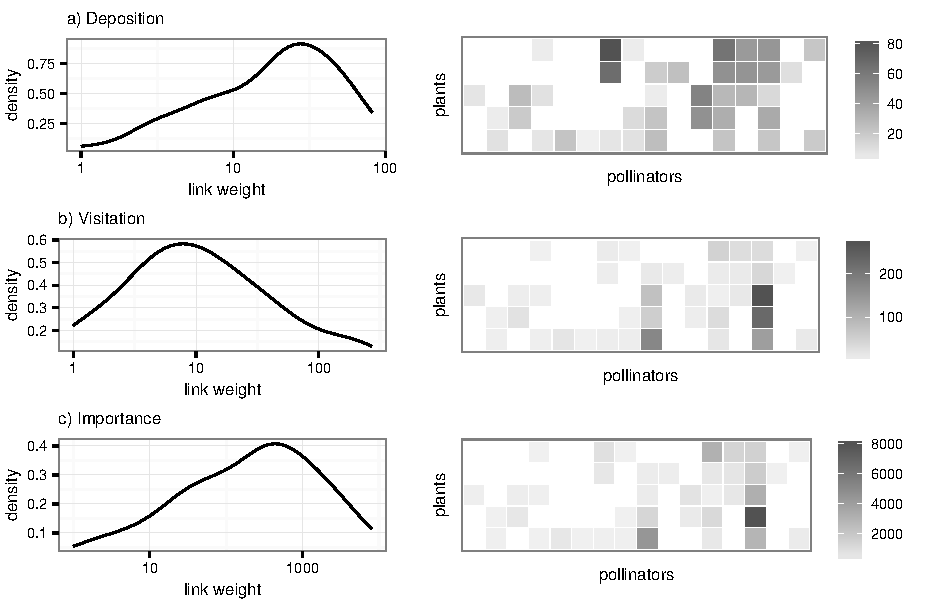
\includegraphics{supp_info_2_files/figure-latex/fig-visitation-vs-deposition-vs-importance-1.pdf}
\caption{\textbf{Distribution of interaction weights for the pollen
deposition, visitation and pollinator importance networks}. Note that
the \emph{x} axis in the density plots have been log-transformed.}
\end{figure}

We first investigated the effects at a network scale. Despite marked
differences in the distribution of weights of the three networks, the
minimum number of driver species to control the whole community was
consistent among the three different approaches (0.33 for deposition,
0.33 for the visitation, and 0.38 for the pollinator importance
network).

The choice of weighting used can also have an impact on the relative
importance of species. Therefore we calculated the frequency that each
species is present in the possible sets of driver species under the
three schemes. Although visitation and deposition produce strikingly
different results, we found a very strong agreement between the order
produced by visitation and importance (Supporting Table 2). Finally, we
investigated whether the asymmetry of mutual dependency, which defines
the direction of control, was consistent among the three possible
weighting schemes. We found again that the direction of the dominant
dependency was maintained was consistent for 95\% of the interactions
weighted by visitation or importance, the two most appropriate metrics
for pollinator and plant dependency (Supporting Table 2).

\begin{table}[ht]
\centering
\begin{tabular}{llll}
  \hline
unweighted & deposition & importance & visitation \\ 
  \hline
- & 0.93 ($<$ 0.001) & 0.85 ($<$ 0.001) & 0.85 ($<$ 0.001) \\ 
  87\% & - & 0.86 ($<$ 0.001) & 0.87 ($<$ 0.001) \\ 
  77\% & 74\% & - & 1 ($<$ 0.001) \\ 
  82\% & 74\% & 95\% & - \\ 
   \hline
\end{tabular}
\caption{\textbf{Correlation of $n_d$ among network weighting schemes}. Spearman correlation coeffcients (with p-value) of the relative importance of species and the percentage of interactions that share the direction of dependency obtained using the three weighting schemes and an unweighted scheme.} 
\end{table}

Altogether, evidence supports the idea that visitation is a suitable
metric to estimate the mutual dependency of species pairs. First, it is
directly related to pollinator foraging. Second, it produces results
consistent, at least within our controllability framework, with plant
reproductive success (as estimated by the importance metric).

\section*{References}\label{references}
\addcontentsline{toc}{section}{References}

\hypertarget{refs}{}
\hypertarget{ref-Alarcon2010}{}
Alarcón, R. (2010). Congruence between visitation and pollen-transport
networks in a California plant-pollinator community. \emph{Oikos}, 119,
35--44.

\hypertarget{ref-Almeida-Neto2011}{}
Almeida-Neto, M. \& Ulrich, W. (2011). A straightforward computational
approach for measuring nestedness using quantitative matrices.
\emph{Environmental Modelling and Software}, 26, 173--178.

\hypertarget{ref-Ballantyne2015}{}
Ballantyne, G., Baldock, K.C.R. \& Willmer, P.G. (2015). Constructing
more informative plant-pollinator networks: visitation and pollen
deposition networks in a heathland plant community. \emph{Proceedings of
the Royal Society B}, 282, 20151130.

\hypertarget{ref-Bartomeus2008}{}
Bartomeus, I., Vilà, M. \& Santamaría, L. (2008). Contrasting effects of
invasive plants in plant-pollinator networks. \emph{Oecologia}, 155,
761--770.

\hypertarget{ref-Bascompte2006}{}
Bascompte, J., Jordano, P. \& Olesen, J.M. (2006). Asymetric
Coevolutionary Networks Facilitate Biodiversity Maintenance.
\emph{Science}, 312, 431--433.

\hypertarget{ref-Bluthgen2007}{}
Blüthgen, N., Menzel, F., Hovestadt, T., Fiala, B. \& Blüthgen, N.
(2007). Specialization, Constraints, and Conflicting Interests in
Mutualistic Networks. \emph{Current Biology}, 17, 341--346.

\hypertarget{ref-Csardi2006a}{}
Csardi, G. \& Nepusz, T. (2006). The igraph software package for complex
network research. \emph{InterJournal, Complex Systems}, 1695, 1--9.

\hypertarget{ref-King2013}{}
King, C., Ballantyne, G. \& Willmer, P.G. (2013). Why flower visitation
is a poor proxy for pollination: Measuring single-visit pollen
deposition, with implications for pollination networks and conservation.
\emph{Methods in Ecology and Evolution}, 4, 811--818.

\hypertarget{ref-Lopezaraiza-Mikel2007}{}
Lopezaraiza-Mikel, M.E., Hayes, R.B., Whalley, M.R. \& Memmott, J.
(2007). The impact of an alien plant on a native plant-pollinator
network: An experimental approach. \emph{Ecology Letters}, 10, 539--550.

\hypertarget{ref-NeEman2010}{}
Ne'Eman, G., Jürgens, A., Newstrom-Lloyd, L., Potts, S.G. \& Dafni, A.
(2010). A framework for comparing pollinator performance: Effectiveness
and efficiency. \emph{Biological Reviews}, 85, 435--451.

\hypertarget{ref-Vazquez2005}{}
Vázquez, D.P., Morris, W.F. \& Jordano, P. (2005). Interaction frequency
as a surrogate for the total effect of animal mutualists on plants.
\emph{Ecology Letters}, 8, 1088--1094.

\end{document}
